\documentclass[12pt]{article}
\usepackage[frenchb]{babel}
\usepackage[utf-8]{inputenc}  %%latin1
\usepackage{fullpage}
\usepackage{graphicx}		%% to insert pics
\usepackage{listings}
\usepackage{color}
\usepackage{url}
\usepackage{pythonhighlight}
\usepackage{hyperref}
\usepackage{xcolor}

\title{Spotify Million Playlist Challenge}
\author{Pablo Schneider - Malte Schwenker - Isa Kilic}

\hypersetup{linkcolor=blue}
\definecolor{medium-blue}{rgb}{0,0,139}
\definecolor{mygreen}{rgb}{0,0.6,0}
\definecolor{mygray}{rgb}{0.5,0.5,0.5}
\definecolor{mymauve}{rgb}{0.58,0,0.82}
\hypersetup{colorlinks, urlcolor={medium-blue}}
\date{02. März 2022}
\lstset{ %
  backgroundcolor=\color{white},   % choose the background color
  basicstyle=\footnotesize,        % size of fonts used for the code
  breaklines=true,                 % automatic line breaking only at whitespace
  captionpos=b,                    % sets the caption-position to bottom
  commentstyle=\color{mygreen},    % comment style
  escapeinside={\%*}{*)},          % if you want to add LaTeX within your code
  keywordstyle=\color{blue},       % keyword style
  stringstyle=\color{mymauve},     % string literal style
}


\begin{document}
\maketitle
\renewcommand{\contentsname}{Inhaltsverzeichnis}

\begin{center}
\tableofcontents
\end{center}
\newpage
\section{Spotify Million Playlist Challenge}

Die Spotify Million Playlist Challenge bezieht sich darauf, per datamining bzw. machinelearning Songs vorschlagen zu können, um Playlists zu vervollständigen. Hierfür gibts sowohl Algorithmische, als auch Logische Lösungswege.

\subsection{Similarity Matrix}
Track-Track similarity Matrix, in welcher Attribute von Tracks verglichen werden, und dann per Ähnlichkeitsanalyse entschieden werden kann, welche Tracks in eine Trackliste passen, um diese zu vervollständigen.

\subsection{Collaborative Filtering}
Collaborative-Filtering basiert auf der Annahme, dass Ähnlichkeiten zwischen den Interessen von Nutzern (hier Playlists) und Produkten (hier Tracks) existiert:

\begin{itemize}
    \renewcommand{\labelitemi}{$\rightarrow}
    \item User-Based um Interessen des Users für das Filtering zu verwenden
    \item Item-Based um Item-Ähnlichkeit (also hier Track-Ähnlichkeit in Playlists) für das Filtering zu verwenden
\end{itemize}


\subsection{Filtern über Trackinfos}
Infos über die Tracks werden über die Spotify API aus den TrackURIs gezogen Es wird kategorisiert und so neu gegliedert - so werden sinnvoll ähnliche Tracks zusammen gruppiert Hierzu zählen beispielsweise Genres wie Zugehörigkeit zu Rock oder Pop, und auch die Danceability (aussagekräftiger als bspw BPM, da BPM auch für die Danceability hinzugezogen wird). Mehr hierzu in \ref{SpoitfyApi}.

\subsection{Assoziationsanalyse - Unser Hauptansatz}
\label{Assoziationsanalyse}
Hier basierend auf dem Apriori Algorithmus. Umgesetzt mit der mlxtend-library und später ergänzt mit dem Frequent Pattern (FP) Growth Algorithmus, der ähnlich, aber für größere Datenmengen schneller, abläuft.\footnote{Agrawal, Rakesh, and Ramakrishnan Srikant. "Fast algorithms for mining association rules." Proc. 20th int. conf. very large data bases, VLDB. Vol. 1215. 1994.}
\\\\
Um die Daten richtig verwenden, und nach dem Apriori Algorithmus gescheit widerspiegeln zu können, müssen diese zunächst sanitized werden.\footnote{\href{https://practicaldatascience.co.uk/data-science/how-to-use-the-apriori-algorithm-for-market-basket-analysis}{How to use the apriori Algorithm for market basket analysis} -- Matt Clark}
\\\\\\\\\\
Zunächst erstellen wir also ein neues DataFrame namens baskets , in welche wir die
Spalten, die wir brauchen zuweisen. 
In unserem Fall sind das playlist\_id und track\_uri.
Nun verwenden wir die Pandas groupby() Funktion um auf beiden Spalten zu gruppieren. Letztlich werden noch mit \color{mymauve}sum \color{black} die Quantitäten-Spalte berechnet, mit \color{mymauve}unstack \color{black} die Hierarchie nach rechts verschoben und mit \color{mymauve}fillna(0) \color{black} alle nan Werte mit 0 gefüllt.
\begin{python}
df2 = df.assign(test=itemQuanity(df['track_uri']))
baskets = df2.groupby(['playlist_id', 'track_uri'])['test'].sum().unstack().reset_index().fillna(0).set_index('playlist_id')
baskets = baskets.applymap(encode_units)
\end{python}
Mit \color{mymauve}applymap(encode\_units) \color{black} werden die Werte auf 1 oder 0 encoded.
\begin{python}
def encode_units(x):
    if x <= 0:
        return 0
    if x >= 1:
        return 1
\end{python}
Als wir aber mit größeren Daten gearbeitet haben, gab es sehr lange Laufzeiten, da das Erstellen der Baskets sehr aufwändig war. Bei der Suche nach Alternativen haben wir letztlich den Transencoder von mlxtend entdeckt.\footnote{\href{http://rasbt.github.io/mlxtend/user_guide/preprocessing/TransactionEncoder/}{Mlxtend transaction encoder}} 
\\\\
Der TransactionEncoder ermöglicht uns ein Dataframe aus einer Liste, welche für alle Playlisten Listen mit Tracks enhalten, zu erstellen. Die Liste müsste dann diese Form: 
\begin{python}
[[track00, .. , track0N], ... ,[trackN0, .. , trackNN]] 
\end{python}\\
\begin{python}
te = TransactionEncoder()
te_data = te.fit(basket).transform(basket)
dfbasket = pd.DataFrame(te_data, columns=te.columns_)
\end{python}
Durch die Anwendung des TransactionEncoder mit der \color{mymauve}fit \color{black} und der \color{mymauve}transform \color{black} Methode wird eine 2D Liste erstellt, in der jeder innere liste die Information enthält, ob diese mindestens einen Träck enthält oder nicht. Mit Hilfe von Pandas erstellen wir dann ein Dataframe.
\\
Jetzt kriegen wir per unserer (most recent) Apriori Implementation\footnote{\href{http://rasbt.github.io/mlxtend/user_guide/frequent_patterns/fpgrowth/}{Frequent Itemsets via the FP-Growth Algorithm}}\footnote{\href{http://rasbt.github.io/mlxtend/user_guide/frequent_patterns/apriori/}{Frequent itemset via Apriori} - Alter Ansatz}:
\begin{python}
itemsets= fpgrowth(basket, use_colnames=True, verbose=0, min_support=0.001, max_len=3)
rules= association_rules(itemsets, metric="lift", min_threshold=1)
rules= rules.sort_values(['confidence', 'lift'], ascending=[False, False])
\end{python}
Regeln mit sowohl Konfidenz-Werten als auch Lift-Werten. Konfidenz-Werte besagen wie "sicher" sich der Algorithmus ist, dass zwei Songs am besten
zusammen vorkommen sollten (bzw. eben zusammen vorkommen). Per diesem Wert sind Songs dann aufeinander (oder an Playlisten) anhängbar.

\section{Vorgehensweise}
Vorgehensweise zum erhalten der Daten, welche für das Ergebnis (submission) nötig ist.

\subsection{Datenextrahierung}
- \color{mygray}DataAnalysis\textbackslash loadSpotifyData \color{black} - \\\\
Zunächst müssen alle relevanten Daten von allen Playlists die relevant sind aus der Datenbank extrahiert werden.\\
Somit müssen die: 
\begin{itemize}
    \item Playlist\_id
    \item Anzahl der Tracks
    \item Kollektion von Tracks in einer Playlist
    \item Position von Tracks in dieser Kollektion
\end{itemize}
per Queries in eine extra CSV Datei (hier die test.csv Kaskade) übertragen werden.
\\

\subsection{Assoziationsregeln erstellen}
 - \color{mygray}DataAnalysis\textbackslash associationRuleMining \color{black} - \\\\
Damit nun aus den in den vorherigem Schritt extrahierten Daten per Apriori Assoziationsregeln erstellt werden können, müssen die Daten in eine Datenstruktur
umfunktioniert werden (aka. Pandas Dataframe). Mehr hierzu in \ref{Assoziationsanalyse}.

\subsection{Assoziationsregeln anwenden und Submission erstellen} 
 - \color{mygray}DataAnalysis\textbackslash submissions \color{black} -\\\\
Um nun letztlich die Submission File erstellen zu können, müssen die Regeln noch angewendet werden. Per Angabe der Aufgabenstellung in der Challenge,
sollten pro Playlist insgesamt \color{mygreen}genau 500 neue Tracks \color{black} vorkommen. Auch Dopplungen von Songs sind nicht erwünscht. Nun wird also für jeden Track in jeder Playlist überprüft, ob ein Track vorkommt, welcher einen anderen Track per Assoziationsregel "zugewiesen bekommen hat". So füllen wir die Playlists dementsprechend auf.

\newpage
\section{Unsere Submissions}

\subsection{Erster Apriori Ansatz}
Bei unserem ersten Apriori Ansatz, haben wir unsere Baskets mit denen wir die Regeln erstellt haben aufgeteilt, um Multi-Processing zu ermöglichen. Dies ist allerdings Kontraproduktiv, da wir somit die einzelnen Samples nicht mehr mit allen Transaktionen vergleichen können. Es kamen also im Vergleich zum zweiten Ansatz viel wenigere Regeln dabei Raus. Dies spiegelt sich auch in der Bewertung unserer Submissions wieder.\\\\
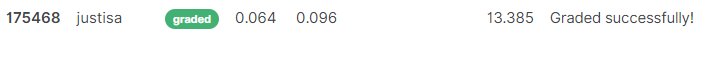
\includegraphics[scale=0.8]{firstSub.png}
\subsection{Zweiter FP-Growth Ansatz}
Da die Performance bei unserem zweiten Ansatz um einiges Akzeptabler war, war es uns Möglich den Algorithmus auf alle Testdaten gleichzeitig laufen zu lassen. Dies hat zu einer verdreifachung unseres Scores geführt.\\
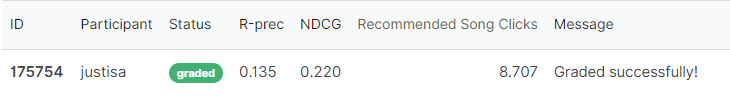
\includegraphics[scale=0.8]{secondSub.png}


\section{Weiterführende Konzepte}
\subsection{Spotify-Api}
\label{SpoitfyApi}
Unsere Submission wird immernoch mit einem relativ niedrigen Score bewertet. Dies liegt vor allem daran, das wir bei leeren Playlists random Tracks einführen. Um dies zu verbessern haben wir den Ansatz verfolgt Metadaten von einzelnen Tracks auszulesen. \\\\
Infos über die Tracks werden über die Spotify API aus den TrackURIs gezogen. Es wird kategorisiert und so neu gegliedert - so werden sinnvoll ähnliche Tracks zusammen gruppiert. Hierzu zählen beispielsweise Genres wie Zugehörigkeit zu Rock oder Pop, und auch die Danceability (aussagekräftiger als bspw BPM, da BPM auch für die Danceability hinzugezogen wird). Diesen Ansatz könnte man über das Content based Filtering noch weiter verfolgen. Hierzu würden die Features zugezogen, und dann Playlists anhand dessen aufgestellt werden. Das hat zeitlich allerdings nicht ganz gereicht.
\\\\
Leere Playlists mit beispielsweise dem Namen "Country" oder "Techno", würden dann mit Songs aufgefüllt werden, denen man diese Genres zugewiesen hat.
\end{document}